\uuid{0wvO}
\exo7id{7745}
\titre{exo7 7745}
\auteur{mourougane}
\organisation{exo7}
\datecreate{2021-08-11}
\isIndication{false}
\isCorrection{true}
\chapitre{Géométrie projective}
\sousChapitre{Géométrie projective}
\module{Algèbre et géométrie}
\niveau{L3}
\difficulte{}

\contenu{
\texte{
Soit $F$ une homographie du plan projectif $P^2$ qui admet une droite $d$ de points fixes.
}
\begin{enumerate}
    \item \question{Montrer qu'on peut choisir $f\in GL(3,k)$ telle que $F=P(f)$ et $f$ admet un plan de points fixes.}
    \item \question{Montrer alors qu'il existe un point $O$ de $P^2$ (appelé centre de $F$) tel que pour tout point $M$ de $P^2$ non fixé par $F$, la droite $(MF(M))$ passe par $O$.}
    \item \question{Soit $d$ une droite et $O$ un point hors de $d$. Soit $A$ et $A'$ deux points hors de $d$ et $A\not=O$ et $O,A,A'$ alignés. Montrer en choisissant un repère convenable qu'il existe une unique homographie $F$ telle que $d$ soit une droite de points fixes et $O$ le centre et qui envoie $A$ sur $A'$.}
    \item \question{Soit $F$ une homographie du plan projectif $P^2$ qui admet une droite $d$ de points fixes et de centre $O$. Sachant que $F(A)=A'$, construire l'image du point $M$ par $F$ dans les cas suivants.
    
    \begin{figure}[!ht] 
        \begin{center}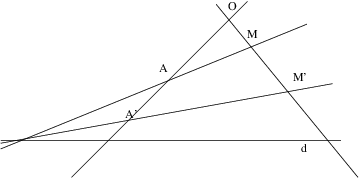
\includegraphics[scale=0.5]{images/img-mour-497-1}\end{center}
        \caption{}
    \end{figure}
    
    \begin{figure}[!ht] 
        \begin{center}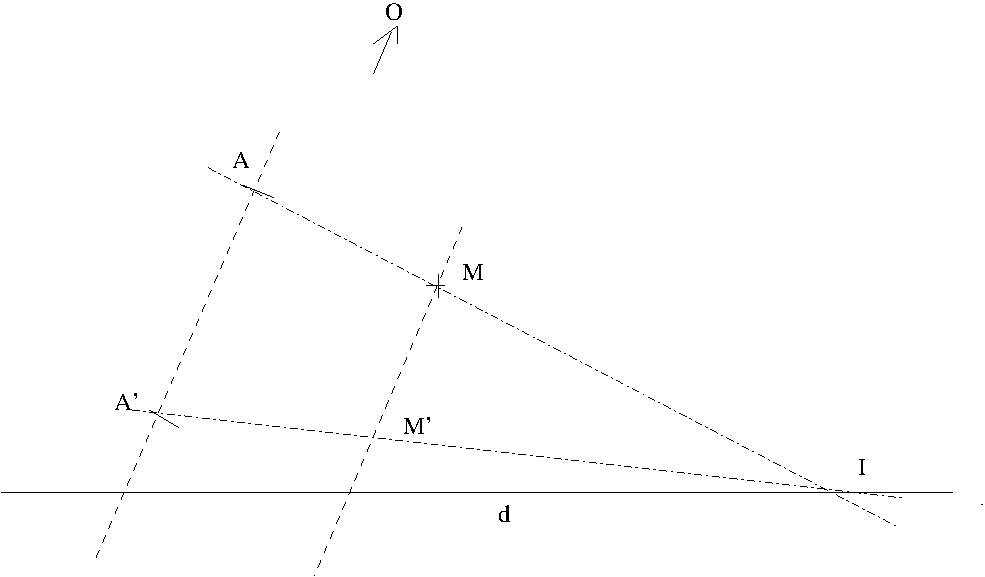
\includegraphics[scale=0.5]{images/img-mour-497-2}
            \caption{le point $O$ est à l'infini}\end{center}
    \end{figure}
    
    \begin{figure}[!ht] 
        \begin{center}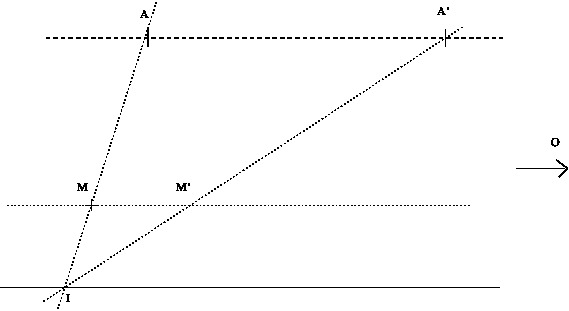
\includegraphics[scale=0.4]{images/img-mour-497-3}
            \caption{le point $0$ est à l'infini dans la direction de $d$}\end{center}
    \end{figure}}
    \item \question{Soit $H$ une involution. On considère deux points $P$ et $Q$ tels que avec leur image $P'$ et $Q'$ ils forment un repère projectif (aucun triplet n'est formé de points alignés).
    On définit $O:=(PP')\cap (QQ')$ et $d$ la droite reliant $(PQ')\cap(QP')$ et $(PQ)\cap(P'Q')$. Montrer que $H$ est l'homographie de droite fixe $d$ de centre $O$ qui envoie $P$ sur $P'$.}
\reponse{
Comme $F$ admet une droite $d$ de points fixes, $f$ fixe toutes les droites d'un plan. C'est donc en restriction à ce plan, une homothétie. Quitte à diviser par ce rapport non nul, on peut supposer que $f$ est l'identité sur ce plan.
L'application $f$ est alors soit une dilatation, soit une transvection. Dans le premier cas, avec un repère adapté, tout point de coordonnées $(X,Y,Z)$ et son image de coordonnées $X,Y,\lambda Z)$ sont coplanaires avec le point de coordonnées $(0,0,1)$.
    Dans le second cas tout point de coordonnées $(X,Y,Z)$ et son image de coordonnées $(X,Y+Z,Z)$ sont coplanaires avec le point de coordonnées $(0,1,0)$.
    On en déduit donc l'existence d'un centre $O$.
On choisit un repère projectif de $P^2$ composé de $M_1$ et $M_2$ sur $d$, puis $M_3=O$ et comme point unitaire $M_4=A$. On obtient un repère tel que $d$ ait pour équation $Z=0$ et $O$ pour coordonnées homogènes $[0:0:1]$ et $A$ pour coordonnées homogènes $[1:1:1]$. Notons $[x:x:z]$ des coordonées homogènes de $A'$ aligné avec $O$ et $A$ avec $x\not=0$ car $A'\not=O$ et  $z\not=0$ car $A'\not\in d$.
    On peut donc normaliser avec $A'[1:1:z]$. Comme $d$ doit être laissée fixe par l'homographie cherchée $P(f)$, quitte à normaliser, on peut supposer que $f$ est l'identité sur $vect(e_1,e_2)$. Comme $P(f)(A)=A'$, $f(e_1+e_2+e_3)=e_1+e_2+f(e_3)$ est proportionel à $e_1+e_2+ze_3$. Donc, $f(e_3)=ze_3$.
    Réciproquement, cette application $f$ satisfait les conditions requises (voir le cas de la dilatation).
\begin{figure}[!ht] 
        \begin{center}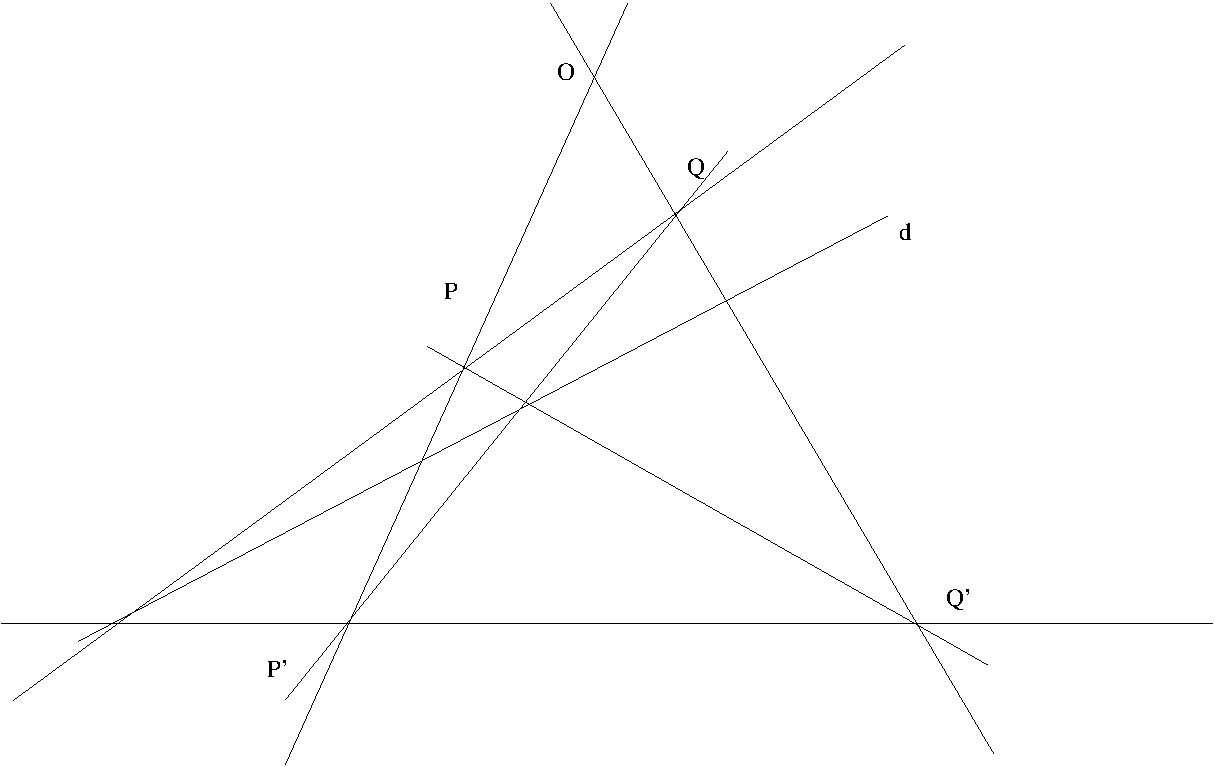
\includegraphics[scale=0.6]{images/img-mour-497-4}\end{center}
        \caption{}
    \end{figure}
    Notons $\phi$ l'homographie de droite fixe $d$ de centre $O$ qui envoie $P$ sur $P'$. On vérifie successivement qu'elle envoie $P$ sur $P'$, $Q$ sur $Q'$, $P'$ sur $P$ et enfin $Q'$ sur $Q$. Elle coïncide avec $H$ sur un repère projectif donc partout.
}
\end{enumerate}
}
